\section{Date: 2026-11-09}
\noindent \textbf{Series ID: DODFFSWCMI} 

\noindent This series is titled Rest of the World; Debt Securities and Loans; Liability, Level and has a frequency of Quarterly, End of Period. The units are Millions of U.S. Dollars and the seasonal adjustment is Seasonally Adjusted Annual Rate.The observation start date is 1945-10-01 and the observation end date is 2026-04-01.The popularity of this series is 15. \\ 

\noindent \textbf{Series ID: PLNSPCEPCHOUSUTL} 

\noindent This series is titled Per Capita Personal Consumption Expenditures: Services: Housing and Utilities for Plains BEA Region and has a frequency of Annual. The units are Dollars and the seasonal adjustment is Not Seasonally Adjusted.The observation start date is 1997-01-01 and the observation end date is 2025-01-01.The popularity of this series is 1. \\ 

\subsection{Raw Regression}
\noindent Regresses the two series against each other directly. A significant result here can come just as easily from both series sharing a long-run trend as from any real relationship.

\begin{center}
\begin{tabular}{lclc}
\toprule
\textbf{Dep. Variable:}          & value\_fred\_PLNSPCEPCHOUSUTL & \textbf{  R-squared:         } &     0.961   \\
\textbf{Model:}                  &              OLS              & \textbf{  Adj. R-squared:    } &     0.959   \\
\textbf{Method:}                 &         Least Squares         & \textbf{  F-statistic:       } &     660.0   \\
\textbf{Date:}                   &        Mon, 09 Nov 2026       & \textbf{  Prob (F-statistic):} &  1.64e-20   \\
\textbf{Time:}                   &            21:41:25           & \textbf{  Log-Likelihood:    } &   -207.55   \\
\textbf{No. Observations:}       &                 29            & \textbf{  AIC:               } &     419.1   \\
\textbf{Df Residuals:}           &                 27            & \textbf{  BIC:               } &     421.8   \\
\textbf{Df Model:}               &                  1            & \textbf{                     } &             \\
\textbf{Covariance Type:}        &           nonrobust           & \textbf{                     } &             \\
\bottomrule
\end{tabular}
\begin{tabular}{lcccccc}
                                 & \textbf{coef} & \textbf{std err} & \textbf{t} & \textbf{P$> |$t$|$} & \textbf{[0.025} & \textbf{0.975]}  \\
\midrule
\textbf{const}                   &    3193.5604  &      115.903     &    27.554  &         0.000        &     2955.747    &     3431.374     \\
\textbf{value\_fred\_DODFFSWCMI} &       0.0008  &     3.03e-05     &    25.690  &         0.000        &        0.001    &        0.001     \\
\bottomrule
\end{tabular}
\begin{tabular}{lclc}
\textbf{Omnibus:}       &  0.836 & \textbf{  Durbin-Watson:     } &    0.483  \\
\textbf{Prob(Omnibus):} &  0.658 & \textbf{  Jarque-Bera (JB):  } &    0.750  \\
\textbf{Skew:}          &  0.053 & \textbf{  Prob(JB):          } &    0.687  \\
\textbf{Kurtosis:}      &  2.219 & \textbf{  Cond. No.          } & 7.43e+06  \\
\bottomrule
\end{tabular}
%\caption{OLS Regression Results}
\end{center}

Notes: \newline
 [1] Standard Errors assume that the covariance matrix of the errors is correctly specified. \newline
 [2] The condition number is large, 7.43e+06. This might indicate that there are \newline
 strong multicollinearity or other numerical problems.

\begin{figure}
\centering
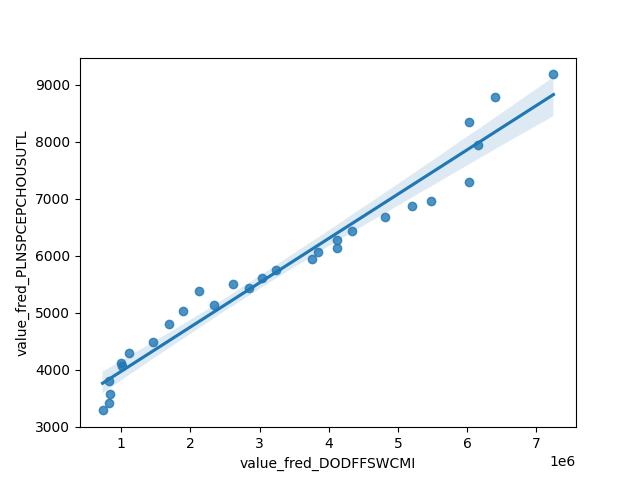
\includegraphics[scale = 0.9]{plots/plot_2026-11-09.png}
\caption{Raw Regression Plot for 2026-11-09}
\end{figure}
\newpage
\subsection{Detrended Regression}
\noindent Regresses the residuals of each series after removing its own linear time trend, so a shared trend can no longer drive the result on its own. A relationship that stays significant here is better evidence of a genuine link between the two series.

\begin{center}
\begin{tabular}{lclc}
\toprule
\textbf{Dep. Variable:}                     & value\_fred\_PLNSPCEPCHOUSUTL\_detrended & \textbf{  R-squared:         } &     0.152   \\
\textbf{Model:}                             &                   OLS                    & \textbf{  Adj. R-squared:    } &     0.121   \\
\textbf{Method:}                            &              Least Squares               & \textbf{  F-statistic:       } &     4.857   \\
\textbf{Date:}                              &             Mon, 09 Nov 2026             & \textbf{  Prob (F-statistic):} &   0.0363    \\
\textbf{Time:}                              &                 21:41:25                 & \textbf{  Log-Likelihood:    } &   -204.23   \\
\textbf{No. Observations:}                  &                      29                  & \textbf{  AIC:               } &     412.5   \\
\textbf{Df Residuals:}                      &                      27                  & \textbf{  BIC:               } &     415.2   \\
\textbf{Df Model:}                          &                       1                  & \textbf{                     } &             \\
\textbf{Covariance Type:}                   &                nonrobust                 & \textbf{                     } &             \\
\bottomrule
\end{tabular}
\begin{tabular}{lcccccc}
                                            & \textbf{coef} & \textbf{std err} & \textbf{t} & \textbf{P$> |$t$|$} & \textbf{[0.025} & \textbf{0.975]}  \\
\midrule
\textbf{const}                              &   -2.367e-12  &       53.276     & -4.44e-14  &         1.000        &     -109.314    &      109.314     \\
\textbf{value\_fred\_DODFFSWCMI\_detrended} &       0.0004  &        0.000     &     2.204  &         0.036        &     2.46e-05    &        0.001     \\
\bottomrule
\end{tabular}
\begin{tabular}{lclc}
\textbf{Omnibus:}       &  1.083 & \textbf{  Durbin-Watson:     } &    0.261  \\
\textbf{Prob(Omnibus):} &  0.582 & \textbf{  Jarque-Bera (JB):  } &    0.897  \\
\textbf{Skew:}          &  0.409 & \textbf{  Prob(JB):          } &    0.638  \\
\textbf{Kurtosis:}      &  2.726 & \textbf{  Cond. No.          } & 3.29e+05  \\
\bottomrule
\end{tabular}
%\caption{OLS Regression Results}
\end{center}

Notes: \newline
 [1] Standard Errors assume that the covariance matrix of the errors is correctly specified. \newline
 [2] The condition number is large, 3.29e+05. This might indicate that there are \newline
 strong multicollinearity or other numerical problems.

\begin{figure}
\centering
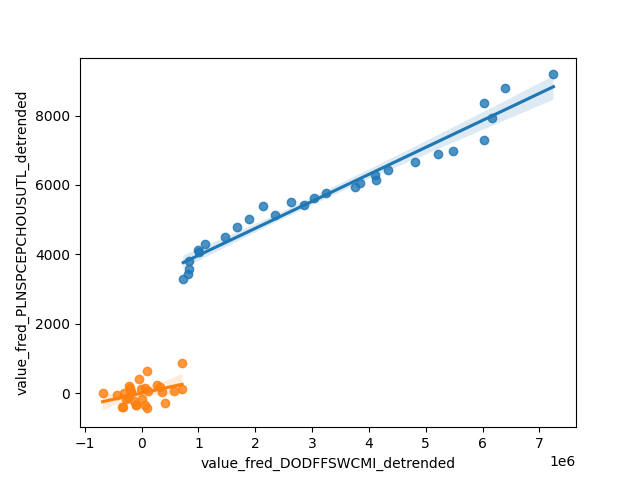
\includegraphics[scale = 0.9]{plots/plot_2026-11-09_detrended.png}
\caption{Detrended Regression Plot for 2026-11-09}
\end{figure}
\newpage
